\chapter{A Quantitative Evaluation of Energy Storage}
\label{chap:battery}

From the previous chapter, I have identified the value of properly sizing energy capacity in an energy harvesting design to increase energy capture and system reliability. 
Many modern energy harvesting sensor designs have utilized capacitors in their designs, which severely limit energy capacity.
Many modern platforms are attempting to push the energy bounds of sensing, computation and networking, and have begun incorporating supercapacitors to provide the necessary energy to make certain applications feasible~\cite{nardello2019camaroptera}.
These decisions are made despite the obvious option for energy capacity: batteries.
%Due to an increased need for energy storage to enable more advanced sensing and processing, the majority of modern batteryless research energy harvesting platforms utilize supercapacitors instead of tantalum or ceramic capacitors due to their superior energy density.
These designers have eschewed batteries as an option, despite their vastly superior energy density, dismissing them qualitatively as 
bulky~\cite{hesterNew17, hesterTragedy15, hesterFlicker17, hesterTimely17, yervaGrafting12, majid2020continuous},
inefficient~\cite{hesterNew17, hesterTragedy15, hesterFlicker17, hesterTimely17},
expensive~\cite{hesterNew17, hesterTragedy15, hesterFlicker17, hesterTimely17, majid2020continuous},
short-lived~\cite{hesterNew17, hesterTragedy15, hesterFlicker17, hesterTimely17, colinReconfigurable18, luciaIntermittent17, yervaGrafting12, majid2020continuous}.
%high-maintenance~\cite{hesterNew17, hesterTragedy15, hesterFlicker17, hesterTimely17, colinReconfigurable18, luciaIntermittent17},
temperature-sensitive~\cite{hesterNew17, hesterTragedy15, hesterFlicker17, hesterTimely17, colinReconfigurable18, luciaIntermittent17},
%difficult to monitor~\cite{hesterNew17, hesterTragedy15, hesterFlicker17, hesterTimely17, colinReconfigurable18, luciaIntermittent17},
%fragile~\cite{hesterNew17, hesterTragedy15, hesterFlicker17, hesterTimely17},
and dangerous~\cite{hesterNew17, hesterTragedy15, hesterFlicker17, hesterTimely17, majid2020continuous}. 
%These qualitative claims against batteries were valid when considering some of the first available rechargeable batteries. 

In this chapter, I reexamine each of these arguments with respect to modern capacitor, supercapacitor, and battery technology. 
While the early battery design of one or two decades ago were certainly guilty of many of the complaints against them, new 
battery electrode materials and improved lithium-ion manufacturing processes have produced appealing options for miniature energy storage 
that do not possess the same negative qualities as older battery technology. 
%These new batteries still possess orders of magnitude more energy density than capacitors and supercapacitors.
New battery technology paired with newly available low power energy harvesting and battery management ICs~\cite{bq25505,adp5091} enables the design of high-capacity energy harvesting systems.
Despite improvements, batteries still underperform in some metrics compared to supercapacitors, but these deficiencies are likely inconsequential for the majority of wireless sensor applications, and the substantial increase in energy capacity outweighs any detracting tradeoffs.\\

\begin{landscape}
\placefigure{tab:battery:cost}
\end{landscape}

\section{Energy Storage Technology}
\label{sec:battery-new}

I summarize the notable characteristics of various examples of capacitors, supercapacitors, and batteries in \cref{tab:battery:cost}. Many of the capacitors and supercapacitors in this table were chosen based on their inclusion in some contemporary batteryless platforms, including the Solar Monjolo~\cite{campbellEnergy14}, Flicker~\cite{hesterFlicker17}, Capybara~\cite{colinReconfigurable18}, and Camaroptera~\cite{nardello2019camaroptera}.
The selected batteries represent some of the smallest lithium-based cells that are commercially available. 
This section serves to explain the characteristics of various possible energy storage technologies for low power energy harvesting applications, as a prelude to deeper dives on particular aspects and comparisons.

\subsection{Ceramic and Tantalum Capacitors}
Along with chip resistors, the multilayer ceramic capacitor (MLCC) is the most widely used passive component in modern electronics. MLCCs are essentially a parallel connection of many cearamic plate capacitors, packaged in a small form factor~\cite{pan2010brief}. Traditionally, MLCCs are used for two applications: resonant circuits and filters and power supply bypass and decoupling~\cite{pan2010brief}. With sufficient capacitance, MLCC capacitors meant for power supply decoupling can act as the sole energy storage in a system~\cite{hesterFlicker17,yervaGrafting12,campbellEnergy14}. However, the energy storage and density of MLCC components is limited, and is often only enough to support a single small operation, like operating a sensor and transmitting the results over a radio. Similarly, tantalum capacitors are often used for power supply bypass and decoupling. Tantalum capacitors consist of a tantalum metal anode and a solid electrolyte as a cathode, separated by a solid dielectric~\cite{gill1994basic}. They generally provide more capacitance per volume than MLCCs, but are polar and have worse efficiency.
Tantalum capacitors also do not exhibit any aging effects, whereas MLCCs experience slight capacitance change over long periods of time~\cite{kemetUpdate}.
Compared to batteries and supercapacitors, MLCC and tantalum capacitors provide infinitely longer lifetimes and higher power density, but are severely limited in energy capacity and density.

\subsection{Supercapacitors}
Electrochemical double layer capacitors (EDLC) are the most common type of supercapacitor, and is utilized in many batteryless platforms~\cite{colinReconfigurable18,libich2018supercapacitors,nardello2019camaroptera}.
Supercapacitors generally consist of electrodes separated by a liquid electrolyte, like batteries, however energy accumulation is through electrostatic interaction instead of chemical reactions~\cite{libich2018supercapacitors,vangari2013supercapacitors}.
EDLCs achieve significantly higher energy density than MLCC and tantalum capacitors due to their large effective surface area and very small charge separation distances. Supercapacitors are also durable and long-lived, capable of millions of cycles~\cite{libich2018supercapacitors}. 
supercapacitors excel in high power, high cycling applications, where large amounts of charge must be stored and provided quickly, at a high frequency.
However, they offer lower power densities due to higher internal resistance compared to MLCC and tantalum capacitors~\cite{vangari2013supercapacitors}. 

\subsection{Li-ion}
Lithium-ion batteries encompass all batteries that utilize lithium ions for charge transfer. These batteries are well known for their superior energy density, and are used in small wireless and portable consumer electronics as well as in large multi-cell configurations in electric vehicles.
Like all batteries, Li-ion batteries consist of two oppositely charged electrodes separated by an electrolyte. The electrodes consist of a negatively charged anode and positively charged cathode. During discharge, Li\textsuperscript{-} ions move from the anode through the electrolyte to the cathode, and during charge they move from the cathode to the anode.
Lithium polymer (Lipo) batteries, most commonly used in consumer electronics, utilize a dry or gel electrolyte, while coin cells or cylindrical Li-ion cells utilize a liquid electrolyte. 

There are many different types of li-ion batteries, utilizing different anode, cathode, and electrolyte materials. Most modern Li-ion cells primarily utilize graphite as an anode material, and lithium nickel manganese cobalt oxide
(LiNi\textsubscript{0.33}Mn\textsubscript{0.33}Co\textsubscript{0.33}O\textsubscript{2} or NMC for short) as a cathode material~\cite{nitta2015li}.
These cells offer a nominal voltage of 3.7\si{\volt}, high energy density, and long lifetimes. 
The choice of NMC provides several benefits over earlier designs that utilize 
LiCoO\textsubscript{2} (LCO) or LiMn\textsubscript{2}O\textsubscript{4} (LMO) for cathode materials.
LCO lithium batteries are notorious for their thermal instability and fast capacity fade at high current rates or deep cycling~\cite{nitta2015li}. 
Cobalt is also a toxic and expensive metal to produce. 
LMO lithium batteries are cheaper, have higher power density, and have significantly better thermal stability than LCO cells, but have lower energy density and still have poor cycling stability, especially at higher temperatures~\cite{nitta2015li}.
The combination of nickel, manganese, and cobalt in NMC cathodes results in higher structural stability, longer lifetimes, and less reliance on expensive transition metals~\cite{nitta2015li}. 

Batteries that utilize LCO cathodes have the propensity to ignite or explode due to thermal runaway when stressed thermally, mechanically, or electrically~\cite{doughty2012general}. This is primarily due to the cathodes releasing oxygen at high temperatures, which start an exothermic reaction with the organic parts of the cell~\cite{doughty2012general, nitta2015li}. Like LCO, the newer NMC cathode material is still susceptible to thermal runaway with abuse, however the peak magnitude of self-heating on runaway is an order of magnitude less than that of LCO, and onset is delayed and begins at a higher temperature~\cite{doughty2012general}.
Batteries with LMO cathodes are safer than both LCO and NMC, but have poor cycle cycling lifetime which has limited the technology's commercialization. 

\subsection{Lithium Iron Phosphate}
Lithium iron phosphate  (LiFePO\textsubscript{4}, or LFP), is a more recently commercialized cathode material and stands to offer similar safety and power capability to LMO while offering long lifetimes similar to NMC~\cite{preger2020degradation, nitta2015li}.
Batteries that utilize LFP as a cathode material possess a lower nominal voltage (3.2\si{\volt}), and lower energy density than LCO and NMC batteries. However, LFP 
cathodes offer higher cycle stability and lifetime, have lower thermal sensitivity, and are cheaper to produce than cobalt and manganese-based cathodes~\cite{doughty2012general,nitta2015li,preger2020degradation}. LFP cells are also very safe compared to NMC and LCO cells. The only thermal runaway experienced by LFP batteries is dominated by reactions between the electrolyte and graphite anode, which decomposes at high temperatures~\cite{doughty2012general}. 

\subsection{Lithium Titanate Oxide}
Perhaps the most promising replacement for graphite anodes is lithium titanate oxide (Li\textsubscript{4}Ti\textsubscript{5}O\textsubscript{4}).
Lithium titanate oxide, abbreviated LTO, is usually paired with an LMO cathode, and sometimes an NMC cathode~\cite{nitta2015li, belharouakElectrochemistry11, sandhya2014lithium}. LTO offers superior thermal stability, high discharge/charge rates, and longer lifetimes compared to graphite. These improvements come at a cost of the more expensive titanium compound, and a lower energy density and nominal voltage (2.4\si{\volt})~\cite{nitta2015li,sandhya2014lithium}. Cells that incorporate LTO anodes are also extremely safe compared to those that use graphite~\cite{nitta2015li, belharouakElectrochemistry11, sandhya2014lithium}. Unlike graphite, LTO anodes do not produce Li dendrites after considerable cycling~\cite{nitta2015li}. This reduces the risk of inadvertent internal shorts and thermal runaway. LTO anodes also remain stable and do not break down at high temperatures~\cite{belharouakElectrochemistry11}.

\subsection{Solid-state}
All cylindrical or pouch Li-ion batteries employ a liquid or gel electrolyte of lithium salts dissolved in an organic, non-aqueous solvent~\cite{doughty2012general}. Liquid electrolyte requires specific packaging to prevent leakage, and an internal separator to prevent shorts between the electrodes. This limits the miniaturization of Li-ion batteries, as this packaging is increasingly difficult to manufacture at smaller sizes. This results in smaller batteries that have uncharacteristically high internal resistance and lower energy density compared to larger cells with the same chemistry.
The organic solvent used in liquid and gel electrolytes also can react exothermically with any oxygen released upon the breakdown of electrode material and cause thermal runaway. In addition to developing new anode and cathode materials to mitigate this, researchers and companies have also begun experimenting with replacing the non-solid electrolyte non-reactive alternatives. Solid-state batteries are safer, due to the use of non-reactive solid electrolytes, come in smaller packages, offer longer lifetimes, and have very low self-discharge~\cite{kim2015review}. However, solid-state batteries generally have limited energy and power density and high internal resistance compared to aqueous Li-ion cells. Solid-state batteries are also currently expensive to manufacture, and their commercial viability has been limited~\cite{kim2015review}.

\subsection{Summary}
Capacitors possess superior power density and have functionally infinite lifetimes, but can only store minute amounts of energy. Supercapacitors provide one to two orders of magnitude more energy density than MLCC and tantalum capacitors, at the cost of reduced power density, and more limited lifetimes. By contrast, batteries offer one to two orders of magnitude more energy density than supercapacitors. However, batteries do have limited lifetimes based on cycle counts, are more temperature sensitive, and some can be dangerous if mishandled. 

In the rest of this chapter, I seek to compare these technologies in more depth. The following sections directly analyze each of the high-level qualitative arguments that "batteryless" platform designers have leveled against batteries. Namely, that they are bulky, inefficient, expensive, short-lived, temperature-sensitive, and dangerous. 


\section{Volume and Density}
\label{sec:battery:density}
Arguments that deride batteries as bulky are likely directly comparing the size of a small battery to that of single tantalum or ceramic capacitor, without considering energy and power density. Modern, commercially available miniature batteries are comparable in volume to many supercapacitors, and even a banked combination of ceramic and tantalum capacitors, while offering substantially more energy density and an acceptable power density. In this section, I explore the "bulkiness" of capacitors, supercapacitors, and batteries in the context of energy and power density. Here, I am considering volumetric density (\si[per-mode=symbol]{\Wh\per\liter}  and  \si[per-mode=symbol]{\watt\per\liter}) instead of specific energy and power (\si[per-mode=symbol]{\Wh\per\kilo\gram} and  \si[per-mode=symbol]{\watt\per\kilo\gram}, respectively) to better compare the volume of these energy storage options. The energy density and power density of various capacitors, supercapacitors, and batteries are directly compared in \cref{fig:battery:ragone}.

\placefigure{fig:battery:ragone}

\subsection{Energy Density}
Energy density should be the primary consideration for energy harvesting power supply design to maximize energy capacity while simultaneously minimizing volume. 
The energy stored in a capacitor is calculated in one of two ways:

$$E_{eff_{cap}} = \frac{1}{2} C (V^2 - V_{min}^2)$$
$$E_{total_{cap}} = \frac{1}{2} C V^2$$

\noindent Where $E_{eff}$ and $E_{total}$ is the effective and total energy stored in a capacitor, respectively. These amounts are defined by the capacitor's capacitance $C$, and the applied voltage $V$, and the minimum voltage $V_{min}$. Usually $V_{min}$ represents the minimum to do something useful. Often this is the minimum open circuit voltage to cold start a boost regulator, between 400\si{\milli\volt} to 600\si{\milli\volt}~\cite{adp5091,bq25505,max17222}. 
For simplicity, I use $E_{total}$ to determine energy capacity and density. For most capacitors, the unusable energy represented by $E_{eff_{cap}}$ is negligible compared to the total energy. Likewise, energy stored in a battery is estimated as follows:

$$E_{bat} \approx Q V_{nom}$$

\noindent Where $Q$ is the charge capacity (often denoted in terms of \si{\Ah}) and $V_{nom}$ is the battery's nominal voltage. Nominal voltage represents an average of the battery's voltage curve over the course of a charge/discharge cycle. The nominal voltage and capacity of a battery are provided by the manufacturer and are almost always included in a datasheet.

A selection of capacitor, supercapacitor, and battery energy capacities and densities are summarized in \cref{tab:battery:cost}, and their energy density is compared in \cref{fig:battery:ragone}. Among this selection, small batteries are 50-1000x more energy dense than supercapacitors and three to five orders of magnitude more dense than ceramic and tantalum capacitors. Li-ion and LiPo batteries are the most energy dense among all options. Solid-state batteries are an order of magnitude less energy dense than those with aqueous electrolytes, but still an order of magnitude more dense than supercapacitors. 

Several of these capacitors, supercapacitors and batteries are shown visually in \cref{fig:battery:sizes}.
The capacitor and supercapacitor configurations are based on examples from batteryless platform designs described in the literature~\cite{hesterFlicker17, campbellEnergy14,colinReconfigurable18}.
The batteries shown in \cref{fig:battery:sizes} are
as small as 88\si{\milli\meter\cubed}, and resemble small through-hole
capacitors and coin cells. Battery \textbf{(b)} is smaller in volume than many of the capacitor
configurations presented in the literature, only outdone by systems like Flicker \textbf{(a)} which utilize only a few ceramic capacitors~\cite{hesterFlicker17}.
This small LTO battery offers 3.7x 
more energy storage and 50x more energy density than the largest supercapacitor presented (\textbf{h}). When considering the size of other components in the system, most notably the harvester (solar panel, thermocouple, or piezoelectric device), the combination of ICs, and large sensors like a PIR motion sensor, the size of small rechargeable batteries is inconsequential. 
To my knowledge, the Michigan Micro Mote is the smallest energy harvesting system, occupying a volume on the order of a single ceramic capacitor~\cite{lee13modular}. Despite its small size, it utilizes a thin film solid-state lithium battery for energy storage due to its superior energy density over any capacitor or supercapacitor option.
When one considers energy density instead of purely volume, capacitors and supercapacitors are significantly more bulky than batteries.

\placefigure{fig:battery:sizes}

\subsection{Power Density}
In addition to energy density, power density is also an important metric to consider for a design. 
Common wireless sensor workloads are characterized by very low sleep currents punctuated by infrequent pulses of high current, usually a radio transmission. Energy storage must provide sufficient peak power to drive these short pulses, but largely, these applications require low continuous power. The maximum peak power is largely dependent on equivalent series resistance (ESR) of the storage device, represented by an internal series resistance to the capacitor or battery cell. 
Internal resistance for both supercapacitors and batteries is temperature and age dependent. Both storage elements experience increased ESR at temperature extremes, and experience increased ESR as they age.
The internal resistance of capacitors and supercapacitors is also frequency dependent, and usually reported for 1\si{\kilo\hertz}. This value is generally related inversely with frequency for frequencies below the capacitor's self-resonance~\cite{murataESRArticle}. For the relatively low frequency of charge/discharge cycles characteristic of energy harvesting devices, actual ESR is likely higher than reported for supercapacitors.

Internal capacitor, supercapacitor, and battery resistance incurs a voltage drop over this resistance which is especially noticeable and detrimental during high  current loads.
Ceramic and tantalum capacitors have negligible ESR and incomparably high power density, so I focus on comparing the power density of supercapacitors and batteries.
There are two different metrics for quantifying power output of supercapacitors and batteries. The first is effective power $P_{eff}$, and represents the maximum sustainable continuous power that can be provided. The second is peak power $P_{max}$ and represents the maximum possible current that can be provided in short pulses. These metrics are defined differently for supercapacitors and batteries. For a supercapacitor, power output is defined as follows~\cite{IEC62391}:

$$P_{eff_{sc}} = \frac{1}{8} \frac{V^2}{R_i}$$
$$P_{max_{sc}} = \frac{1}{4} \frac{V^2}{R_i}$$

\noindent Where $V$ is the voltage applied to the capacitor, and $R_i$ is the internal resistance, or ESR. For batteries, these metrics are defined as follows:

$$P_{eff_{bat}} = I_{cont} V_{nom}$$
$$P_{max_{bat}} = I_{max} V_{nom}$$

\noindent Where $I_{cont}$ and $I_{max}$ are the battery's rated continuous and peak pulsed current respectively. These metrics are provided by the battery manufacturer and often included in the battery datasheet. The continuous and peak currents are often defined in terms of the C-rate, or a proportion of the rated capacity (in units of \si{\Ah}). For example, the 1C rate of a 100\si{\milli\Ah} battery is 100\si{\milli\ampere}, and the 2C rate is 200\si{\milli\ampere}. 
Continuously charging and discharging a battery beyond its normal rate will result in cycles that deliver less energy than rated, and eventually damage to the cell resulting in capacity fading. 
For sake of comparison, I use $P_{eff}$ in \cref{tab:battery:cost} for batteries and supercapacitors, as it is a more conservative measure of the energy storage power capability. 

Among the supercapacitors and batteries featured in \cref{tab:battery:cost}, supercapacitors provide 10-400x higher power density over batteries. 
However, one supercapacitor outlier provides the least power density of all options. Like energy density, power density is also directly compared in \cref{fig:battery:ragone}.
Despite their superior power density, most applications do not require the higher power density afforded by supercapacitors. 
It is hard to imagine a \textit{low power} energy harvesting application that must source more than a few to a few hundred \si{\milli\ampere} at 3\si{\volt} infrequently, never mind continuously. 
Solid-state batteries are more power limited than other battery types. Despite their low energy capacity they are able to supply high C-rates, between 15-50C. This corresponds to currents on the order of 10\si{\milli\ampere}.
Conventional Li-ion and LiPo cells can generally source 1C continuously. The smallest Li-ion cell listed in \cref{tab:battery:cost} can provide 11\si{\milli\ampere} continuously, and the largest can provide 80\si{\milli\ampere}. The LiPo cell presented can supply 40\si{\milli\ampere} continuously. 
Small LTO and LFP cells are capable of very high C-rates, often between 20-40C for LTOs, and 10-20C for LFP~\cite{lifepo4Datasheet,LTODatasheet,LTODatasheet2}.
The smaller LTO battery listed in \cref{tab:battery:cost} is able to source 18\si{\milli\ampere}, while the larger LTO and LFP cells can source between 400-700\si{\milli\ampere} continuously. 
This power capability is more than sufficient for the majority of applications, either indoors with PANs, or outdoors, with cellular or LPWANs~\cite{nrf52840,ghena2019challenge}.

Another consideration for power capability and ESR is the effect of voltage drops during high power loads. If a voltage drop is sufficiently large, it can drop the supply to a level unusable by a voltage regulator or CMOS logic. This could effectively render part of the power storage unusable in an unpredictable manner. This effect is particularly detrimental for supercapacitors. While ESR is comparable between batteries and supercapacitors, the stability of provided voltage is not. Batteries provide a stable voltage curve centered around their nominal voltage, and voltage drops due to ESR can still result in a usable voltage even when almost empty. Supercapacitors, on the other hand, experience a (approximately) linear decrease in voltage with current until empty. This means that, depending on the load (in intensity and frequency), a large load and subsequent voltage drop could occur that causes a system brown-out, potentially corrupting state, or an unexpected reset. 


\section{Efficiency}
\label{sec:supercapvbattery}
At a high level, the efficiency of an energy storage element can be defined as the actual proportion of stored energy that is used to perform a desired task or application. Batteries have been derided as "inefficient" by batteryless platform designers, however
both supercapacitor and battery technology exhibit the same two phenomena that causes inefficiency, and generally to the same extent. 
The first phenomena is power dissipation over the internal resistance of the device. The second is self-discharge or leakage, which is represented by an internal parallel resistance to the capacitor or battery.
This section seeks to quantitatively compare these two sources of inefficiency for supercapacitors and batteries.

\subsection{Internal Resistance}
The power dissipated over the internal resistance, or ESR, of an energy storage element can be calculated as follows:

$$P_{i} = R_{i} I^2$$

\noindent Due to the squared relationship of power to current, high current loads, such as a radio transmission or long computation, are the primary cause of ESR power losses. The total power required to drive a load, including losses over internal resistance, can be defined as:

$$P_{total} = P_{l} + P_{i}$$
$$P_{total} =  I V + R_{i} I^2$$

\noindent Where $P_l$, $I$ and $V$ are the power, current, and voltage required to drive an intended load. Power inefficiency due to ESR can be very costly when considering high current loads.

With a subset of the capacitors and batteries mentioned in \cref{tab:battery:cost}, an 8\si{\milli\ampere} BLE
transmission from a steady 3\,V would incur less
than 0.03\% in resistive loss from a tantalum capacitor, a 2.1\% loss from the 1.8\si{\milli\Ah} LTO battery, and 6.3\% loss from the 7.5\si{\milli\farad} supercapacitor. A 130\si{\milli\ampere} LoRa transmission would incur a 0.43\%, 25\%, and 52\% overhead, respectively~\cite{ghena2019challenge}. These selections represent some of the worst performing examples in terms of ESR. 
For most supercapacitor and battery product lines, as they get smaller, capacitance and capacity decreases while ESR increases. When the surface area between cell electrodes decreases, this limits the flux of ions traveling between electrodes. This is manifested as an increased internal resistance.
This has traditionally been an issue for small Li-ion batteries. However, the recent commercialization of new manufacturing processes and new cathode and anode materials that increase electrode surface area has led to small form factors with lower ESR, on the order of 1-2\si{\ohm}~\cite{millibatNimbus}. Current solid-state battery technology still struggles with ESR, with values at or above 100\si{\ohm}~\cite{stEnfilm,tdkCeraCharge}.
In \cref{tab:battery:cost}, there are several batteries and supercapacitors that exhibit much lower ESR, on the order of 1\si{\ohm} or less, and are thus more efficient with high current loads. 
The 20\si{\milli\Ah} LTO battery is in the same product line as the 1.8\si{\milli\Ah} cell, but has 15x less ESR. This cell would only incur a 0.15\% and 2.3\% loss on the respective BLE and LoRa transmissions.
%For high current loads, it is very important to not only pick a storage element that can support the load, but one that also has a low internal resistance to energy wasted over the internal resistance. 
Generally, there are options for both supercapacitors and batteries that offer comparable ESR efficiency. %In this respect, batteries \textit{are not} inefficient.


\subsection{Self-Discharge}
In addition to an internal series resistance, capacitors and batteries both feature a non-ideal parallel resistance that causes a continuous self-discharge.
The self-discharge of supercapacitors and batteries is generally dependent on their size and temperature. Larger capacity/capacitance batteries and capacitors from the same product line will exhibit more self discharge than smaller ones. 

The batteries selected in \cref{tab:battery:cost} typically exhibit less than 500\si{\nano\ampere} self-discharge in standard environmental conditions. Solid-state batteries exhibit even less self discharge, at similar rates to capacitors. Notably, many types of Li-ion and LiPo batteries also require additional protection circuitry to prevent deep discharges and overcurrent charging/discharging. This additional circuitry incurs additional self-discharge. However, extremely efficient options exist to manage small batteries~\cite{ltc4071Datasheet,bq25505,adp5091}. The LTC4017 requires only 550\si{\nano\ampere} when in operation, and features a very low disconnect current (<1\si{\nano\ampere}) to extend shelf-life~\cite{ltc4071Datasheet}.
This amount of self-discharge is negligible when considering the average sleep currents of common sensors and MCU options. Generally, sleep currents will still be dominated by memory retention and low frequency clock operation, on the order of a few \si{\micro\ampere}. 

While the self discharge of capacitors and supercapacitors appears lower than batteries, this is partially due to how it is measured and rated. However, the self discharge of supercapacitors is actually is comparable to that of batteries when considering short term post-charge behavior.
Supercapacitors exhibit a pronounced, non-ideal phenomena known as dielectric absorption~\cite{kundert2008modeling}. Dielectric absorption represents a decreasing exponential decay of the supercapacitor voltage immediately after charging. After hours or days, self-discharge is dominated by a linear leakage current. The magnitude of the decay depends on the initial voltage, temperature, and duration of the charge~\cite{kowal2011detailed}. Datasheets generally specify supercapacitor leakage after a subsequent 24 hour constant voltage charge and 1 hour open circuit period. This is sufficient time for the contribution of dielectric absorption to be rendered negligible. After this time, only the internal parallel leakage resistance is a factor.

In the short term, however, the discharge due to dialectric absorption dominates. For example, after an hour of constant voltage charging, the 33\si{\milli\farad} BestCap supercapacitor listed in \cref{tab:battery:cost} experiences an average of 300\si{\nano\ampere} self-discharge over a 3 hour window. Considering the common use case of supercapacitors in batteryless systems, where any captured energy is immediately used whenever it is available. This short term cycle use case means that energy is never stored for an extended period of time, and dialectric absorption is a primary factor in self-discharge for batteryless systems. While I have not characterized the self-discharge of each individual supercapacitor listed in \cref{tab:battery:cost}, this phenomena is inherent to electrochemical capacitor technology.

%In addition to additional leakage due to absorption effects, some batteryless sensor designs employ a bank of multiple parallel capacitors and supercapacitors to build up enough energy storage to support their workload~\cite{colinReconfigurable18}. Since these capacitors are in parallel, their internal resistances are summed. 

Generally, one can expect the short-term self-discharge of supercapacitors to be comparable with batteries. In either case, self-discharge is not sufficient to warrant discounting either option for a low power design. When considering the impact of self-discharge with that of ESR loss, there are suitable options from both technologies that would provide satisfactory performance.

\placefigure{fig:battery:eperd}

\section{Expense}
\label{sec:battery:cost}
Like the bulkiness argument, the claim that batteries are "expensive" is only valid when directly comparing the cost of a battery to that of single ceramic or tantalum capacitor. This view is reductionist, and this section seeks to explore this argument in more detail.

Most batteries are actually comparatively cheap when considering energy capacity and density. 
A single battery provides significantly more energy storage per dollar than any capacitor, supercapacitor, or banked configuration.
\Cref{fig:battery:eperd} illustrates this by comparing the energy per dollar one can expect from capacitors, supercapacitors, and batteries. 
Solid-state batteries are still costly, as they are a newly commercialized technology and their manufacture is still expensive. 
Despite this, solid-state batteries offer a similar magnitude of energy capacity per dollar to supercapacitors.
Other battery types offer several orders of magnitude more energy capacity per dollar than capacitors and supercapacitors.

The expensiveness of capacitors is accentuated when considering that some designs require multiple parallel capacitors or supecapacitors to build up enough energy capacity to enable required atomic operations. For example, the Capybara design is configured with 14 of the 7.5\si{\milli\farad} Seiko supercapacitors, each costing ~\$2.42 USD, for a total of \$33.88~\cite{colinReconfigurable18}. The small 1.8 \si{\milli\Ah} battery offers 4.4x the energy capacity of the combined 14 parallel supercapacitors, for only \$1.25.
It would require 61 of the Seiko supercapacitors to provide the same amount of energy capacity as the 1.8\si{\milli\Ah} battery. Those 61 supercapacitors would cost \$148.

Besides the Seiko supercapacitor, several of the selected supercapacitors in \cref{tab:battery:cost} are as expensive or more expensive than the selected batteries~\cite{murataCap,kemetCap,seikoCap,bestCap}.
Small, 2-50~mAh LTO batteries can be purchased for
\$6.75 USD each from US distributors and \$1.25 USD each from Chinese manufacturers, even in small quantities~\cite{LTODatasheet, LTODatasheet2}. 

%and the
%cost of other key components in an energy harvesting system, like the
Also, when considering the cost of other components in a wireless energy harvesting system, like
an SoC~\cite{nrf52840}, harvester~\cite{sanyoSolarCell} and sensors~\cite{si7021},
which each cost around \$5 USD each in low quantities, a battery will not constitute
the driving cost. Batteries are by far the most cost effective option for providing energy capacity. The argument that they are too expensive for a sensor design says nothing to the comparable cost of supercapacitors, and entirely ignores the benefits of the superior energy density of batteries. 


\section{Lifetime}
Batteries are often considered "short-lived" due to their limited cycle lifetimes, especially when compared to ceramic and tantalum capacitors. 
Ceramic and tantalum capacitors lifetimes are estimated to be thousands to millions of years with proper voltage derating and when used at room temperature~\cite{kemetLife}. 
The lifetime of capacitors, supercapacitors, and batteries generally refers to the lifetime before the device experiences parametric failure. Parametric failure is when the device is no longer within specification, usually when rated capacitance/capacity is lower than 20\% its original value, or when ESR or other parasitics are sufficiently higher than rated.
This section serves as an effort to quantify and compare battery lifetime with capacitors and supercapacitors, and to investigate methods for elongating their cycle lifetimes.
While modern battery technology will never compete with the longevity of capacitors, for low power energy harvesting, cycle lifetime is unlikely to be the limiting factor on the lifetime of a battery, never mind the system as a whole. 

%Perhaps the primary reason for the excitement around batteryless platform is the claim of infinite lifetimes of their power supplies. And this claim has merit when considering ceramic and tantalum capacitors, 
While ceramic and tantalum capacitors can potentially last a million years, these lifetime estimates do not hold for supercapacitors, which are often rated in thousands of hours at a specified voltage and temperature (often 65-85\si{\celsius})~\cite{bestCap,murataCap}. This lifetime is further influenced by the cycling characteristic and intensity of the workload~\cite{kreczanik2013study}. For low power wireless sensors in room temperatures, with the sporadic cycling rate of an intermittent system, one can still expect lifetimes of a hundred thousand to one million hours~\cite{kreczanik2013study}. While this is a long lifetime, it is by no means infinite.

Conversely, the cycle lifetime of a battery is generally the number of full cycles at a rated continuous discharge/charge current (usually 0.5C or 1C) before the battery's capacity diminishes to 80\% of its original rated capacity.
Generally, NMC lithium batteries offer a cycle lifetime between 3000 and 5000 cycles~\cite{richter2017measurements,preger2020degradation}, compared to 300-700 cycles for LCO and LMO batteries.
For small form factor batteries, this cycle lifetime is less, and for those in \cref{tab:battery:cost}, they offer only 300-500 cycles~\cite{lipoDatasheet, millibatNimbus} at a 0.5~C charge/discharge rate.
However, new battery chemestries like LTO and LFP batteries offer between 2000 and 7000 cycles at 0.5~C~\cite{hallExperimental18, LTODatasheet, LTODatasheet2,omarLithium14, sarasketaCycle15, wangCycle11,lifepo4Datasheet, preger2020degradation}. Solid-state batteries also offer long cycle lifetimes, between 1000 and 4000 cycles for commercially available cells~\cite{stEnfilm,tdkCeraCharge}.

These rated cycle lifetimes represent the cycle life at 100\% depth-of-discharge (DoD), however battery cycle lifetime is heavily influenced by the rate of discharge, as well as the depth of discharge.
The reduction of battery DoD to 10\%
exponentially reduces cycle capacity loss, resulting in potential
lifetimes of greater than 10,000 cycles before reaching 20\% capacity degradation with LFP cells~\cite{omarLithium14, wangCycle11}. Similarly, LTO cells are estimated to sustain approximately 15,000 cycles before reaching 20\% capacity degradation~\cite{stroe2018accelerated}.
These cycle estimations for LTO cells hold true even for relatively high temperatures (50-60\textdegree
C)~\cite{wangCycle11, stroe2018accelerated}.
LTO chemistries can be expected to survive one thousand
cycles at 100\% DoD at 55\textdegree C~\cite{han2014cycle}.
Life cycle
expectations for both 100\% and 10\% DoD are summarized in
\cref{tab:battery:cost}.

On its face, several thousand cycles does not seem like a lot compared to the lifetime estimates of capacitors and supercapacitors. However, for batteries, this cycle lifetime amounts to a significant amount energy. This energy also represents a significant amount of time when considering the energy capacity of batteries, and the expected charge/discharge behavior of energy harvesting wireless sensors.
The comparatively vast energy capacity of batteries means that each cycle represents a significant amount of energy. This amount of energy can drive a low power workload for an extended period of time. For example, the representative periodic workload described in \cref{tab:capacity:rep} requires an average power of 58.6\si{\micro\watt}. For the smallest 1.8\si{\milli\Ah} battery, a single discharge cycle represents just over 3 days of continuous operation. The rated 7000 cycle lifetime of this cell represents 117 years, assuming an identical charge/discharge cycle. 

For wireless sensor workloads, battery cycle lifetime is not going to constitute the main source of failure in designs that incorporate them. Instead, limited shelf-life and poor battery management are likely to be the driving forces behind usable battery lifetimes. 
Shelf-life represents the amount of time a battery can sit uncharged before depleting itself and experiencing capacity degradation. Batteries must also be properly charged and discharged within rated current limits, and should not be overvolted or undervolted. 
It is conceivable that energy harvesting systems may be deployed in areas with little available harvestable energy, and be unable to charge their batteries for long periods of time. 
The shelf-life for lithium-based batteries is approximately one decade, however, LTO chemistries have been shown to exhibit no long-term cell
damage when undervolted, even to zero volts~\cite{brunell2016effect}.
This is a significant improvement over traditional technologies like LCO, LMO, and NMC which suffer capacity degradation if undervolted due to long storage and absence of charging. 
Regardless of the type of battery, designs should utilize the myriad of small battery charger and management ICs that exist to properly manage battery state and minimize the effects of shelf-life~\cite{ltc4071Datasheet,bq25505,adp5091}.

The lifetime of an energy harvesting system is also not solely dependent on the lifetime of its power supply.
Most notably, some components exhibit significant long-term calibration drift. For example, each year a humidity sensor~\cite{si7021} expects a quarter of a percent relative humidity drift, while an oscillator~\cite{txc-oscillator} expects 3~ppm drift.
There is also the question of relevancy in the face of decades of future
progress in networking, processor efficiency, and MEMS sensors. At some point, the wireless sensor platforms built today
will be obsolete and less useful, regardless of their theoretical lifetimes. Sensors do not need to last indefinitely, they need to last long enough and provide enough
benefit to justify their original deployment. Replacement and renovation is inevitable.
Conservatively, rechargeable batteries have the capability to last between 10 and 20 years when managed properly. While not cycle limited, supercapacitors have similar lifetime estimates on the order of ecades. 
When considering this reality, only systems that employ ceramic and tantalum capacitors can claim to support indefinite lifetimes. 
%It is unclear that supercapacitor-based batteryless systems are any better off in terms of lifetime than battery-based systems.

\section{Temperature Sensitivity}
In addition to lifetime considerations, batteries are also notorious for their temperature sensitivity. As mentioned previously, in temperature extremes, batteries exhibit higher ESR, self discharge, and have accelerated capacity degradation. Out of the many arguments against batteries, temperature sensitivity is the most coherent. This section seeks to quantify and compare the temperature sensitivity of capacitors, supercapacitors, and batteries and identify the applications for which it has a significant impact.

Ceramic and tantalum capacitors are very temperature resistant. Of the few selected in \cref{tab:battery:cost}, both types are rated for -55 to +125\si{\celsius}~\cite{ceramicDatasheet,ceramicDatasheet2,tantalumDatasheet}. The ceramic and tantalum capacitors both exhibit approximately 10\% capacitance difference at -55 and 85\si{\celsius}. Extreme temperatures can reduce operational lifetimes, however. High temperatures can reduce expected lifetimes from 4000 years at 45\si{\celsius} to just 14 years at 85\si{\celsius} for tantalum capacitors~\cite{kemetLife}.

Supercapacitors are also rated for extreme temperatures, and those listed in \cref{tab:battery:cost} can withstand temperatures between -40 to -20\si{\celsius} on the low end to up to 70\si{\celsius}. Supercapacitors generally experience increased ESR with lower temperatures, and lifetime limits with higher temperatures~\cite{murataCap,bestCap,kreczanik2013study,murataTech}. Capacitance is generally affected by low and high temperatures. For the 33\si{\milli\farad} BestCap, at -40\si{\celsius}, ESR can increase to 20x its rated value. Similarly for the 470\si{\milli\farad} Murata capacitor, it can experience 8x its rated ESR at the same temperature. All supercapacitors have a rated lifetime in terms of hours at a specific temperature. The BestCap can withstand 1000 hours at 70\si{\celsius}, and the Murata cell is rated for 1000 hours at 85\si{\celsius} before experiencing a capacitance degradation of 20\%. For supercapacitors, the effects of extreme temperatures is actually quite severe. At cold temperatures, supercapacitors will be unable to supply current at a sufficient voltage, and at high temperatures their rated lifetime can decrease from hundreds of thousands of hours to just 1000, or from approximately 11 years to 40 days. Even a moderately high temperature of 45\si{\celsius} can reduce some supercapacitor operational lifetimes to 3 years from 14 years at room temperature~\cite{kreczanik2013study}.

Like supercapacitors, batteries experience adverse effects at extreme temperatures. At low temperatures, lithium-based batteries exhibit a reduced energy capacity, support lower charge and discharge rates, exhibit higher ESR, and can experience accelerated shelf-life and cycle aging~\cite{jaguemont2015lithium}. For a LFP battery at -20\si{\celsius}, its capacity is reduced to approximately 60\% of its original value. When this battery is stored at -20\si{\celsius} for 17 days, it experiences a further 10\% capacity degradation to 50\%, and a 16x increase in ESR to 8\si{\milli\ohm} from 0.5\si{\milli\ohm}~\cite{jaguemont2015lithium}.
If charging rates are exceeded at cold temperatures, or the battery is simply cycled at low temperatures, additional battery capacity degradation can occur. The same LFP battery as above experiences a 12\% degradation after only 12 cycles at -20\si{\celsius}~\cite{jaguemont2015lithium}.
Likewise, at higher temperatures, lithium batteries also experience accelerated aging and increased internal resistance~\cite{leng2015effect}. At extreme temperatures, some types of lithium batteries can experience thermal runaway and cause explosions or fires. These effects are rarely described and quantified in battery datasheets. Instead, manufacturers simply provide a range of operational temperatures.

Li-ion and LiPo batteries are particularly sensitive to temperature. Of those listed in \cref{tab:battery:cost}, they are generally only rated for 0-40\si{\celsius} for charging, and -20-60\si{\celsius} for discharging. I would expect them to perform worse than the metrics listed previously for the LiFeMnPO\textsubscript{4} battery.
Generally, LTO and LFP batteries perform better in extreme temperatures than traditional Li-ion and LiPo cells.
Some 
datasheets and authors report operating LTO batteries successfully as low as -30\,\textdegree C
and as high as 75\,\textdegree C~\cite{LTODatasheet2, lifepo4Datasheet, chenEvaluation15}. From their datasheet, the selected LTO cells in \cref{tab:battery:cost} exhibit a 10\% capacity degradation at -20\si{\celsius}, and a 20\% degradation at -30\si{\celsius}. At high temperatures, these cells only experience a 2\% degradation at 75\si{\celsius}, and less than 1\% at 60\si{\celsius}. LFP cells perform worse than LTO cells at lower temperatures. According to the datasheet of the cells in \cref{tab:battery:cost}, they experience 40\% capacity degradation at -20\si{\celsius}, which is in agreement with the previous section~\cite{lifepo4Datasheet, jaguemont2015lithium}. Solid-state batteries also perform relatively well in extreme temperatures due to their solid electrolyte, and there are commercial options rated for -20 to 80\si{\celsius}. However, at -20\si{\celsius}, effective capacity is reduced to just 20\% of original. For this solid-state battery, effective capacity actually increases at 80\si{\celsius} to 120\%~\cite{tdkCeraCharge}.
No information is given on temperature's effect on ESR and long-term cycle lifetime for these cells, but related work indicates these metrics would still be severely impacted by extreme temperatures.
~\cite{wangCycle11, swierczynskiInvestigation14}.

Regardless of type, lithium batteries should be kept as close to room temperature as possible, and in extreme environments like high altitudes, deserts, or even in space or close to the earth's mantle, batteries will require active heating or cooling to maintain an operational lifetime. For example, the Mars Curiosity and Perseverance rovers utilize a Radioisotope Thermoelectric Generator (RTG) to both provide heating and constant thermocouple harvesting to charge a bank of two Li-ion batteries~\cite{nasaPerseverance}. Battery packs with included (non-RTG) heaters are also commercially available for cubesat applications~\cite{nanopowerbpx}.

Batteries are not as robust as capacitors and supercapacitors when used in extreme temperatures, and will require temperature control. However, 
supercapacitors also require active temperature management to maintain long lifetimes at high temperatures. When considering common use cases for wireless sensors, the efficient and operational range of both batteries and supercapacitors encompasses all applications located in spaces that humans occupy, and likely will handle most of the range of temperatures outdoors in many locations.

\section{Safety} 
Besides temperature sensitivity, many types of lithium metal batteries are also notorious for their propensity to burn and explode under mechanical, electrical, and thermal stress.
Capacitors and supercapacitors do not exhibit same caliber of danger, and at most will "pop" if exposed to electrical stress like overcharge or a large inverted charge. 
For both batteries and supercapacitors, electrical stress is exceedingly rare for low power energy harvesting applications, especially if using a battery protection and voltage management circuit. However, in some extreme environments, mechanical and thermal stress can be an issue. 

Batteries with LCO and NMC cathodes and graphite anodes are prone to fiery explosions if mishandled. However, 
batteries that use other electrode materials, like LFP cathodes or LTO anodes, are considered much safer~\cite{doughty2012general,nitta2015li,belharouakElectrochemistry11,larssonAbuse14}.
Compared to LCO and NMC, LFP has enhanced safety and stability~\cite{larssonAbuse14}. The structure of the LFP cathode is more thermally and chemically stable.  
The LFP cathode material has been shown to not release oxygen during thermal runaway, even when fully decomposed at high temperatures. 
The P-O bond within the PO\textsubscript{4}\textsuperscript{3-} ion is stronger than that of the Co-O bond in the CoO\textsubscript{2}\textsuperscript{-}, so that when abused, oxygen is released slowly or not at all~\cite{nitta2015li}.
This results in a significantly safer cell, where any thermal runaway is dominated by anode and electrolyte reactions at extreme temperatures~\cite{doughty2012general}.

Like LFP cathodes, LTO anodes provide similar benefits over graphite anodes. Graphite is prone to expansion and contraction during charging and discharging, respectively, which causes internal damage to the cell, resulting in capacity fading and in rare cases, short circuit conditions~\cite{sandhya2014lithium}. This effect is further exacerbated at extreme temperatures. 
LTO is considered a zero-strain material, meaning it experiences very little change in its chemical structure during charging, discharging, or temperature changes, unlike graphite. When heated to high temperatures, graphite can break down and react exothermically with the electrolyte, releasing flammable hydrocarbons. By contrast, at the same high temperatures, LTO anodes do not produce heat or release any gasses~\cite{belharouakElectrochemistry11}. Beyond the anode chemical stability, the high potential of LTO anodes prevents lithium dendrites from forming upon deep cycling or after many cycles~\cite{nitta2015li}. Lithium dendrites are the main cause for internal shorts in batteries with graphite anodes. These features of LTO anodes greatly lower the risk of internal short circuits, thermal runaway, and explosions.
The solid electrolyte in solid-state batteries also substantially improves safety. A solid electrolyte is not flammable, and since it is solid, it is chemically unable to interact explosively with a decaying cathode or anode~\cite{kim2015review}.

While there is still slight potential for danger under abuse conditions for LTO, LFP, and solid-state batteries, the danger is substantially less than traditional graphite and cobalt-based lithium batteries. For LTO batteries, the danger of thermal runaway and explosion should be equivalent with that of a supercapacitor. Solid-state batteries should be even safer than supercapacitors, as EDLC supercapacitors employ an aqueous electrolyte.
The battery manufacturer for the LTO and LFP cells listed in \cref{tab:battery:cost} states in the datasheet that no battery protection circuit is necessary to ensure safety~\cite{LTODatasheet,LTODatasheet2}. 
These cells also feature a capacitor-like notched cap that fails first in the case of internal pressure and gas release.
Despite their safety, battery management is still important to limit damage to any battery and maintain capacity and performance. 
Not all lithium batteries are equivalent, and the claim that \textit{all} batteries are dangerous disregards the many safety improvements made with newer electrode and electrolyte materials.

\section{Summary}
Among the various arguments that "batteryless" platforms have levied against batteries, very few are relevant in the face of improved battery technology. Out of all addressed here, temperature sensitivity is the only real limitation of batteries. This complicates their usage in extreme environments, but by no means discounts them. Batteries can not compete against some supercapacitors in terms of power density and cycling performance, but for low power applications, these metrics are inconsequential. 
In reality, batteries are by far the most energy dense rechargeable storage device available and they provide many orders of magnitude more energy capacity per dollar than any capacitor or supercapacitor. New battery technology provides comparable efficiency, lifetime, and safety to many modern supercapacitors. 

These qualitative arguments are the same made in the early 2000s, when battery technology was admittedly not well suited for long-lived, low power applications. Two decades later, these arguments have not been revisited, and are instead used ad nauseam to further justify design decisions made to enable theoretically indefinite lifetimes. 
%It has resulted in a lazy or intentionally obtuse view of energy harvesting system design research, where no thought is given to properly sizing components to optimally enable an application. 
%Instead, the decision to use a supercapacitor is the default, chosen to make an application work, but not work well. Research in this area has pivoted from trying to solve interesting and hard problems with wireless sensor networks, to creating complex and overbearing software solutions to shoehorn supercapacitors into applications they are poorly suited for. The real problem is in reality a hardware one: these platforms do not have enough energy capacity. There is also very simple hardware solution: \textbf{use a battery}. 
The choice to use a (super)capacitor has become the default, often selected to provide just enough energy storage to allow an application to function, but nowhere near enough to function well. This lack of energy capacity in the name of immortality has forced researchers to develop complex software and hardware solutions and shoehorn capacitors and supercapacitors into applications they are poorly suited for. There is a far simpler solution: \textbf{use a battery}.

\begin{definetable*}{tab:battery:cost}
    \begin{adjustbox}{width=1.3\textheight}
    \begin{threeparttable}
    \begin{tabular}{l | l | S[table-format=1.9,table-align-text-post = false] | c | S[table-format=3.3,table-align-text-post = false] | S[table-format=7.3,table-align-text-post = false] | S[table-format=3.3,table-align-text-post = false] | c | r | c | c | c | c | c}
     \multirow{2}{*}{Technology}  & {Capacitance / } &  {Energy Capacity} & {Voltage} & {Volume} & {Energy Density} & {Power Density\tnote{b}} & Temperature & ESR &  Self-Discharge &  \multicolumn{2}{c|}{Cycle Life (Cycles)\,\tnote{j}} & \multicolumn{2}{c}{Cost (USD)}\\\cline{11-14}

     & {Capacity} & {(\si{\Wh})} & {(\si{\volt})} &  {(\si{\mm\cubed})} & {(\si[per-mode=symbol]{\Wh\per\liter})} & {(\si[per-mode=symbol]{\watt\per\liter})} & (Charge/Discharge\,\textdegree C) & (\si{\ohm}) & (\si{\nano\ampere}) &  100\% DoD & 10\% DoD & US\,\tnote{m}  & China  \\
      \hline
      
\multirow{2}{*}[0.6em]{MLCC}
    & 47\si{\micro\farad}~\cite{ceramicDatasheet2}  
    & 0.000000259\,\tnote{a}
    & 6.3
    & 8.19 
    & 0.032
    & 6060000\,\tnote{c}
    & -55 - 125
    & 0.001-0.1\,\tnote{f}
    & <10\,\tnote{h}
    & $\infty$\,\tnote{k}
    & $\infty$\,\tnote{k}
    & 0.16
    & 0.03  \\
    
    & 100\si{\micro\farad}~\cite{ceramicDatasheet}
    & 0.00000139\,\tnote{a}
    & 10
    & 20.0
    & 0.069
    & 6250000\,\tnote{c}
    & -55 - 125
    & 0.001-0.1\,\tnote{f}
    & <10\,\tnote{h}
    & $\infty$\,\tnote{k}
    & $\infty$\,\tnote{k}
    & 0.31
    & 0.04  \\
                                
\multirow{2}{*}[0.6em]{Tantalum}    
    & 100\si{\micro\farad}~\cite{tantalumDatasheet}
    & 0.000000551\,\tnote{a}
    & 6.3
    & 18.6
    & 0.030 
    & 2670000\,\tnote{c}
    & -55 - 125 
    & 0.2\,\tnote{f} 
    & <10\,\tnote{h}                        
    & $\infty$\,\tnote{k}         
    & $\infty$\,\tnote{k}   
    & 0.28          
    & 0.17  \\
                                    
    & 220\si{\micro\farad}~\cite{tantalumDatasheet}
    &0.00000306\,\tnote{a}
    & 10
    & 91.0
    & 0.034
    & 1370000\,\tnote{c}
    & -55 - 125      
    & 0.07\,\tnote{f}                    
    & <10\,\tnote{h}                        
    & $\infty$\,\tnote{k}         
    & $\infty$\,\tnote{k}   
    & 0.37          
    & 0.16  \\\hline

\multirow{2}{*}[0.6em]{Supercapacitor}        
    & 7.5\si{\milli\farad}~\cite{seikoCap}   
    & 0.0000704\,\tnote{a}
    & 2.6
    & 7.2               
    & 0.980   
    & 4690
    & -30 - 70\,\tnote{d}               
    &    25\,\tnote{f}                  
    & <10\,\tnote{i}                        
    & >10000                  
    & \textemdash       
    & 2.42
    & {\textemdash}     \\
                                    
    & 33\si{\milli\farad}~\cite{bestCap}
    & 0.000139\,\tnote{a}
    & 5.5
    & 870
    & 0.159
    & 17400
    & -20 - 70\,\tnote{d}               
    & 0.25\,\tnote{f}
    & <5\,\tnote{i}
    & \textemdash             
    & \textemdash
    & 8.65
    & {\textemdash} \\
                                    
    & 100\si{\milli\farad}~\cite{kemetCap}
    & 0.000420\,\tnote{a}
    & 5.5 
    & 1130
    & 0.372
    & 33.5
    & -25 - 70\,\tnote{d}               
    & 100\,\tnote{f} 
    & <10\,\tnote{i}                        
    & \textemdash             
    & \textemdash       
    & 1.10
    & {\textemdash}     \\
                                   
    & 470\si{\milli\farad}~\cite{murataCap}  
    & 0.00115\,\tnote{a}
    & 4.2
    & 1029 
    & 1.17
    & 16500
    & -40 - 70\,\tnote{d}  
    & 0.13\,\tnote{f}
    & <1000
    & 100000+/4\,yr~\cite{murataTech}\,\tnote{l} 
    & \textemdash\,\tnote{l}   
    & 5.06 
    & 1.00  \\\hline
    
\multirow{2}{*}[0.6em]{Li-ion}        

    & 11\si{\milli\Ah}~\cite{millibatNimbus}
    & 0.0407
    & 3.7
    & 191
    & 213
    & 96.9
    & 0 - 40/-20 - 60\,\tnote{f}
    & 1\,\tnote{g}
    & \hl{XX}
    & 500
    & 10000+~\cite{guenaDepth06, millnerModeling10}
    & 4.00
    & \textemdash \\
    
    & 40\si{\milli\Ah}~\cite{40mahliion}
    & 0.148
    & 3.7
    & 1010
    & 147 
    & 44.4
    & 0 - 40/-20 - 60\,\tnote{f}
    & 3
    & 120-400~\cite{zimmermanSelf04}
    & 500
    & 10000+~\cite{guenaDepth06, millnerModeling10}
    & 1.62
    & \textemdash \\
    
    & 80\si{\milli\Ah}~\cite{millibatNimbus}
    & 0.296
    & 3.7
    & 1010
    & 295
    & 147
    & 0 - 40/-20 - 60\,\tnote{f}
    & 2\,\tnote{g}
    & \hl{XX}
    & 500
    & 10000+~\cite{guenaDepth06, millnerModeling10}
    & 7.00
    & \textemdash \\\hline
    
\multirow{2}{*}[0.6em]{LiPo}        
    & 40\si{\milli\Ah}~\cite{lipoDatasheet}
    & 0.148
    & 3.7
    & 660
    & 224
    & 224
    & 0 - 40/-20 - 60\,\tnote{f}
    & 1.5
    & 120-400~\cite{zimmermanSelf04}
    & 300
    & 10000+~\cite{guenaDepth06, millnerModeling10}
    & 4.50
    & 0.51  \\\hline
    
\multirow{2}{*}[0.6em]{LTO}

    & 1.8\si{\milli\Ah}~\cite{LTODatasheet2}
    & 0.0043
    & 2.4
    & 88.0
    & 48.9
    & 489
    & -35 - 70\,\tnote{f}
    & 8  
    & <300\,\tnote{g} 
    & 2000      
    & 10000+~\cite{hallExperimental18}
    &  {\textemdash}& 1.28  \\
    
    & 20\si{\milli\Ah}~\cite{LTODatasheet,LTODatasheet2}
    & 0.0480
    & 2.4
    & 682
    & 70.4
    & 1410 
    & -35 - 70\,\tnote{f}
    & 0.55\,\tnote{g}
    &  <300\,\tnote{g}
    & 7000
    & 10000+~\cite{hallExperimental18}
    & 6.75
    & 1.28  \\\hline
    
LFP
    & 70\si{\milli\Ah}~\cite{lifepo4Datasheet}
    & 0.224
    & 3.2
    & 1570 
    & 143
    & 1430 
    & -20 - 75\,\tnote{f}
    & 0.18
    & \hl{160}~\cite{swierczynskiInvestigation14}
    & 2000
    & 30000+~\cite{wangCycle11,sarasketaCycle15,omarLithium14}
    &  {\textemdash}
    & 1.28 \\\hline

Solid State
    & 0.7\si{\milli\Ah}~\cite{stEnfilm}
    & 0.00273
    & 3.9
    & 145
    & 18.8
    & 134.2
    & -20 - 60\,\tnote{f}
    & 100
    & <3
    & 4000
    & {\textemdash}
    & 30.00 
    & {\textemdash} \\
    
    & 0.1\si{\milli\Ah}~\cite{tdkCeraCharge}
    & 0.000150
    & 1.50
    & 14.5
    & 10.3
    & 2.07
    & -20 - 80\,\tnote{f}
    & <200
    & <80
    & 1000
    & {\textemdash}
    & 9.31
    & {\textemdash} \\
    
%\multirow{2}{*}[0.6em]{Li-Primary}  & 720\,mWh~\cite{primary2032}    & 1005\,\tnote{a}  & 716               & -30 - 60\,\tnote{f}               & {N/A\,\tnote{i}}          & 250                                   &N/A                      &  N/A              & 0.20          & 0.10  \\
%                                    & 4500\,mWh~\cite{primarycr123a} & 7830\,\tnote{a}  & 574               & -40 - 70\,\tnote{f}               & {N/A\,\tnote{i}}          & 1400                                  &N/A                      &  N/A              & 0.90          & 0.75  \\
%\multirow{2}{*}[0.6em]{Li-Thin Film}& 3.9\,mWh~\cite{thinDatasheet}  & 119              & 32.7              & -20 - 60\,\tnote{f}               & 80                        & 3.5                                   &4000                     &\textemdash        & 18.24         & {\textemdash}     \\
%                                    & 190\,\textmu Wh~\cite{thinDatasheet2} & 58        & 3.2               & -40 - 70\,\tnote{f}               & 2200                      & 0.2                                   &300                      &  5000             &  {\textemdash}& {\textemdash}     \\
   \end{tabular}
    \begin{tablenotes}[para]
        \item[a] Energy capacity calculated with rated maximum voltage.
        \item[b] Calculated with battery and capacitor effective power. \\
        \item[c] Effective power for capacitors is slightly nebulous. Here the higher end of ESR is assumed.
        \item[d] Supercapacitors experience higher ESR at lower temperatures and higher leakage at higher temperatures~\cite{murataTech}.\\
        \item[e] Lithium batteries experience higher ESR, higher leakage, lower capacity and shorter lifetimes at temperature extremes.
        \item[f] ESR is frequency dependent, supercapacitors are usually rated at 1\si{\kilo\hertz}. \\
        \item[g] Empirically tested.
        \item[h] Both tested and calculated from insulation resistance after absorption period.
        \item[i] Specification after 24\,h of charging.
        \item[j] For batteries, measured to 80\% original rated capacity.
        \item[k] Capacitor derating is not considered. With proper design principals these should be nearly infinite.
        \item[l] Supercapacitors are time rather than cycle limited. Assumes 3V, 20\,\textdegree C. No DoD dependence mentioned~\cite{murataTech}. \\
        \item[m] Prices are based on cheapest available equivalent part in quantities of 100.
    \end{tablenotes}
    \end{threeparttable}
    \end{adjustbox}
    \caption{A comparison of miniature energy storage technologies.
    \normalfont
    Data is based on specific components and their datasheets, and
    components are chosen for each category based on their inclusion in platforms described by the literature.
    Some technologies are rapidly evolving, such as supercapacitors and batteries. Other citations point to general characteristics 
    of the storage technologies not specified by their datasheets. For
    most applications, lithium-based batteries provide much higher energy density
    without reasonably impacting sensor lifetime, cost, or function.
    The minority of sensing applications, such as those operating at extreme
    temperatures, may require capacitors or active heating and cooling.}

\end{definetable*}

\begin{definefigure}{fig:battery:sizes}
  \centering
  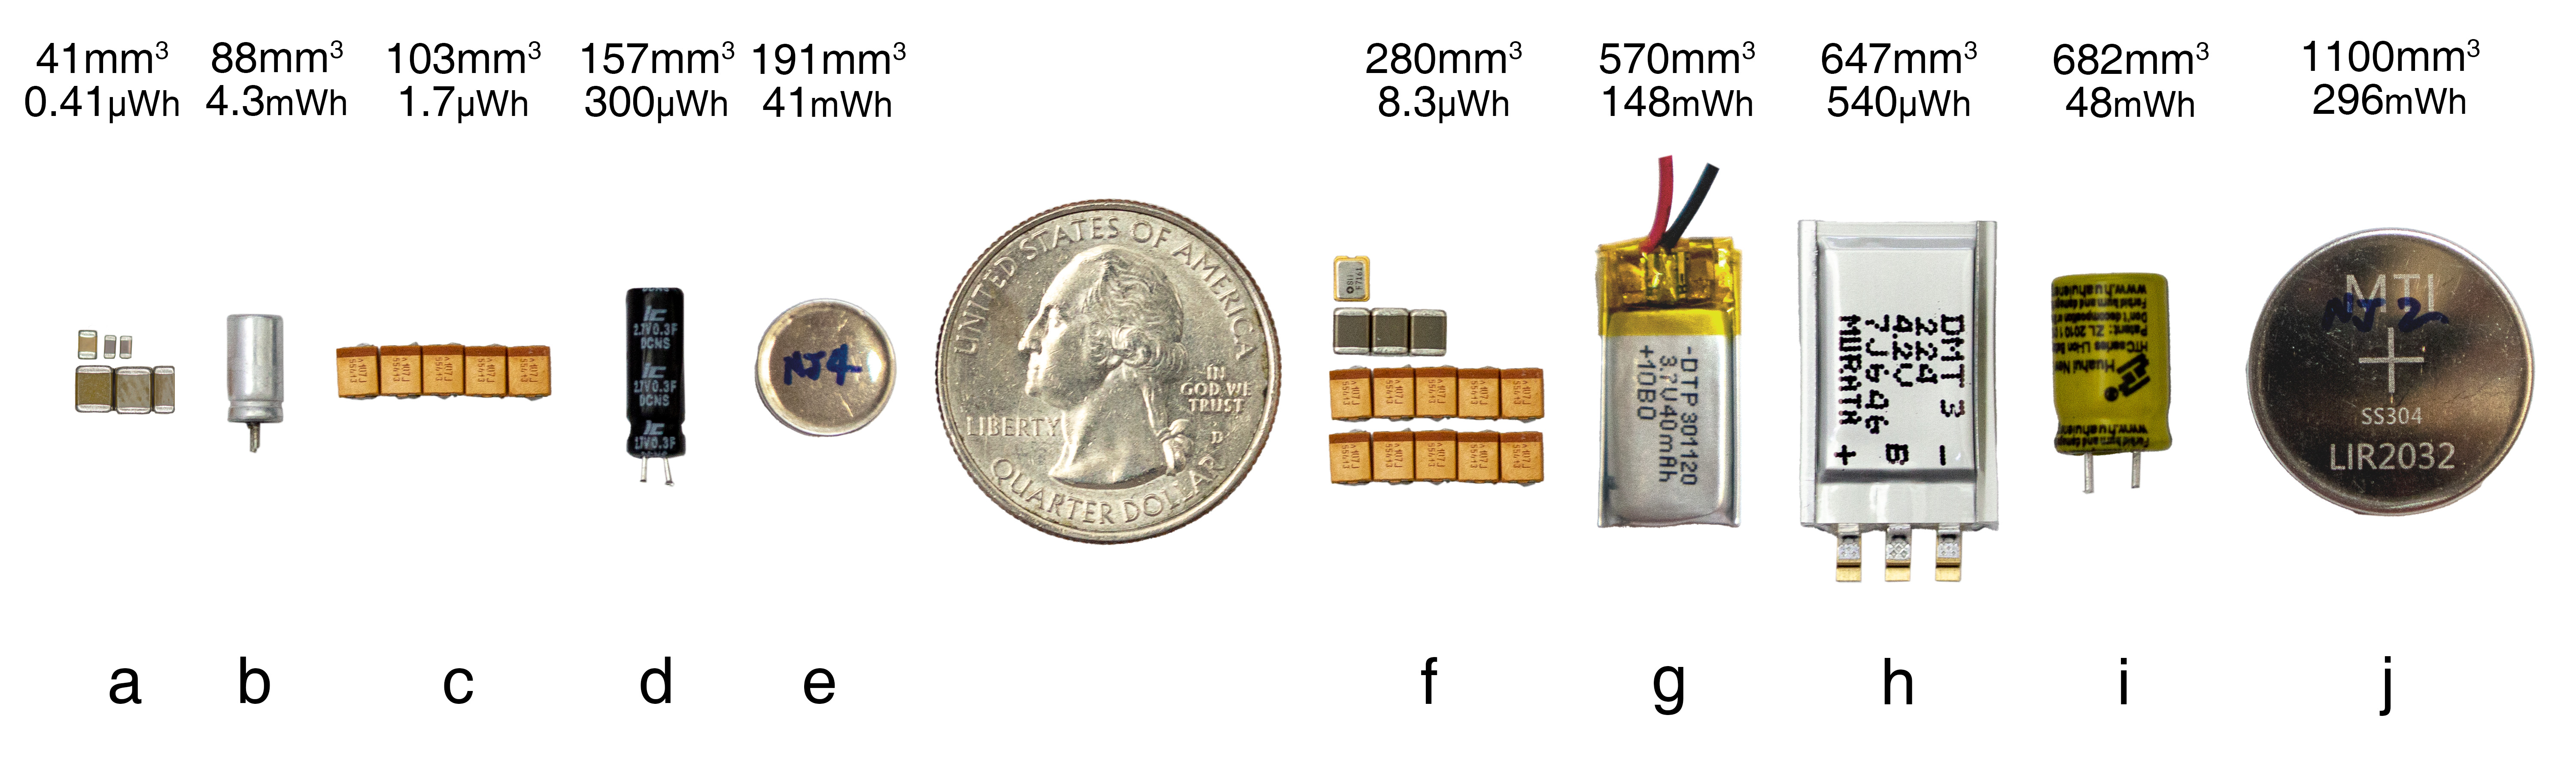
\includegraphics[width=\columnwidth]{figs/batteries/cap_lto_size_compare}
  \caption{
    A size comparison of energy storage methods including capacitors, supercapacitors, and batteries.
    \normalfont
    They are ordered left to right, by their
    (total) volume. Total volumes and energy storage are listed above the respective device.
    Configuration
    \textbf{(a)}, \textbf{(c)} and \textbf{(f)} represent the energy storage configurations used
    in the Flicker platfrom with BLE and several sensors~\cite{hesterFlicker17}, the Solar Monjolo~\cite{campbellEnergy14} and the Capybara temperature
    monitor and alarm~\cite{colinReconfigurable18}, which have total
    capacitances and energy capacities of 119\si{\micro\farad} (0.41\si{\micro\Wh} at 5~V), 500\si{\micro\farad} (1.7\si{\micro\Wh} at 5~V)
    and 8.8\si{\milli\farad} (8.3\si{\micro\Wh} at 2.6~V), respectively. Capacitors
    \textbf{(d)}~\cite{illinoisCap} and \textbf{(h)}~\cite{murataCap} are large
    supercapacitors available on the Capybara platform and have the
    capacitances and energy capacities of 300\si{\milli\farad} (300\si{\micro\Wh} at 2.7\si{\volt}) and 220\si{\milli\farad}
    (540\si{\micro\Wh} at 4.2\si{\volt}) respectively.  Devices \textbf{(b)} and \textbf{(i)} are 
    small LTO battery cells with 1.8\si{\milli\Ah} (4.3\si{\milli\Wh} at 2.4~V) and 20\si{\milli\Ah} (48\si{\milli\Wh}
    at 2.4\si{\volt}) capacity respectively~\cite{LTODatasheet2}. Devices \textbf{(e)} and \textbf{(j)} are small prototype Li-ion coin cells with 11\si{\milli\Ah} (41\si{\milli\Wh} at 3.7~V) and 80\si{\milli\Ah} (296\si{\milli\Wh} at 3.7~V) respectively~\cite{millibatNimbus}. Device \textbf{g} is a traditional Lithium Polymer pouch cell with 40\si{\milli\Ah} (148\si{\milli\Wh} at 3.7~V)~\cite{sparkfunPouch}.
    The LTO battery \textbf{(b)} and the Li-ion coin cell \textbf{(e)} are among the smallest of all configurations of energy storage
    presented here and also provide one to two orders of magnitude more energy capacity
    compared to \textbf{(f)}, the largest supercapacitor presented.
  }
\end{definefigure}

\begin{definefigure}{fig:battery:ragone}
\centering
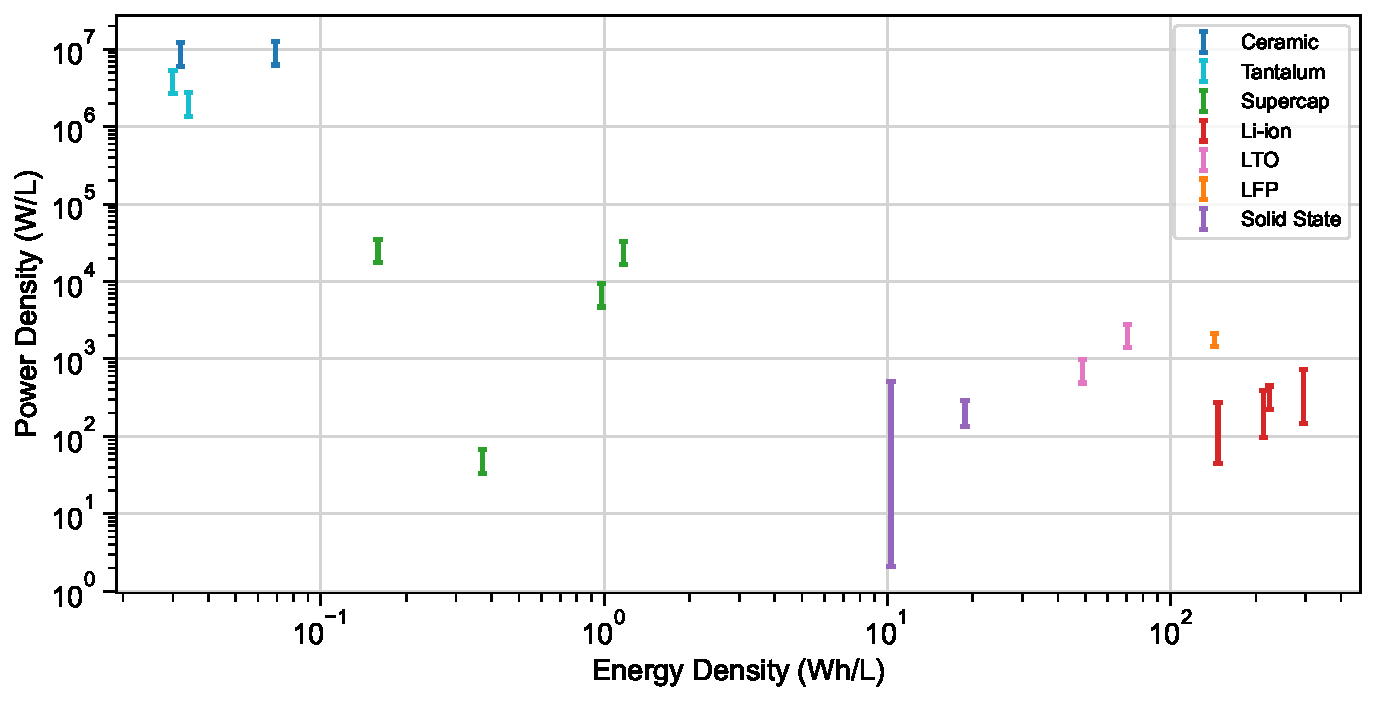
\includegraphics[width=\columnwidth]{figs/ragone}
\caption{Ragone plot for components listed in \cref{tab:battery:cost}, in log-log scale. A ragone plot directly compares power and energy density for different devices. Ceramic and tantalum capacitors are very power dense, but provide abysmal energy density. Batteries provide superior energy density, are less power dense. Supercapacitors exist between these two extremes. Even though batteries do not provide comparable power density to either capacitors or supercapacitors, they can still provide sufficient power for common wireless sensor workloads, like operating a short or long range radio.}
\end{definefigure}

\begin{definefigure}{fig:battery:eperd}
\centering
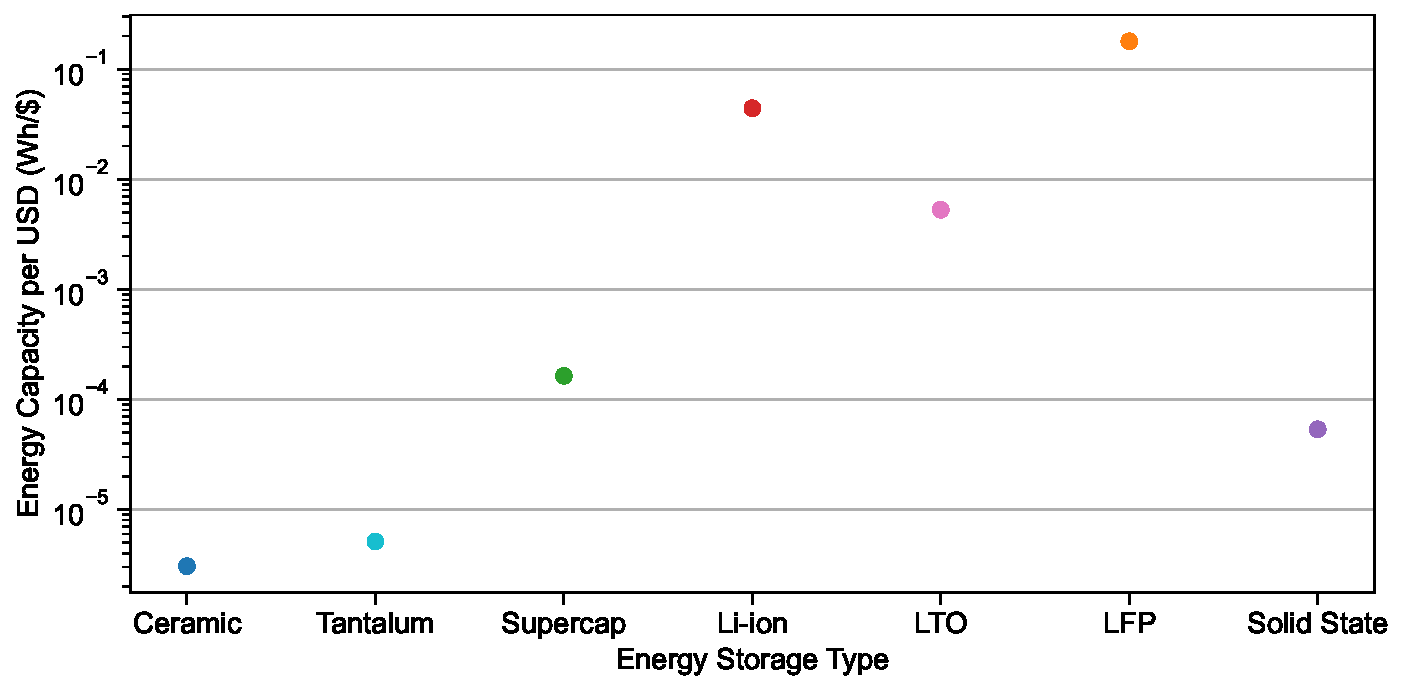
\includegraphics[width=\columnwidth]{figs/energy_per_cost.pdf}
\caption{
    Average energy capacity for various technologies selected in \cref{tab:battery:cost}, normalized by price in USD. Wherever possible, component costs were determined by their price in the United States. In regards to energy capacity, batteries offer 3-5 orders of magnitude more energy capacity per dollar than ceramic and tantalum capacitors. Batteries also offer 2-3 orders of magnitude more capacity than supercapacitors.
}
\end{definefigure}
